\chapter{Literature Review}
%SL: Add a little more here to tell the reader what they should expect to see in the section. 

This section will discuss the background literature relating to this research project. This will include an introduction to supervised machine learning and classification with a focus on text classification. 
A significant amount of research has been carried out in classifying tweets, particularly classifying the sentiment of tweets. The techniques used for tweet classification and sentiment classification will be explored. Finally some of the current approaches to hotel recommendation will be presented.

\section{Classification}

Classification, in the context of machine learning, is the process of mapping observations into classes, based on some set of training data. There are two main approaches to classification, supervised and unsupervised learning. 

Supervised machine learning \cite{supervised2007} involves labelled data. There are input variables (x) and output variables (y) and an algorithm is used to train the mapping function from the input to the output (y = f(x)). The mapping function that has been trained is then applied to new unseen data to decide it's class. Supervised machine learning algorithms include Support Vector Machines \cite{Vapnik1995,Vapnik21995}, Naive Bayes Classifiers \cite{NaiveBayes1998}, Random Forest Classifiers \cite{Breiman2001}, Decision Tree Classifiers \cite{decisionTrees1991}, Logistic Regression Classifiers \cite{logisticRegression2007} and Nearest Neighbour Classifiers \cite{knn2001}. 
%SL: why no references for the last few?

Unsupervised machine learning uses unlabelled data. It only has input variables (x) with no output variables. The learning algorithm is used to identify patterns directly from the data. There are no predefined classes. Unsupervised learning is used to discover unknown patterns in data. Unsupervised machine learning algorithms include K-Means Clustering \cite{kmeans2002} and Gaussian Mixture Models \cite{}. 
%SL: again, a reference if possible

A supervised machine learning approach will be taken in this research. A collection of tweets will be manually annotated and assigned one of the following three labels: Review, Some Content, or Irrelevant. These annotated tweets will be used to train a text classifier. 
%SL: user whatever wording you provided to the participants 

\section{Text Classification}

Text classification is one application of both supervised and unsupervised machine learning \cite{khan2010}. Classification algorithms can be applied to a wide range of different areas, which include text, speech, images and video. In this research we are attempting to classify the text found in tweets. Certain classification algorithms are more suited to classifying text. Text classification involves automatically assigning a set of classes to raw text documents. Applications include sentiment analysis, spam detection, language detection and topic classification. This section will discuss the functionality of some classification algorithms that are suited to text classification. 

%Some popular text classification algorithms are Support Vector Machines, Naive Bayes Classifiers, Logistic Regression Classifiers, Maximum Entropy Classifiers, Decision Tree Classifiers and Ensemble Classifiers. In this section, the functionality of these text classification algorithms will be discussed.

%SL: you already list these as classification approaches, above. Perhaps outline why you are discussing text classification separate to classification and how these approaches differ from the more generic classifiers 

A Support Vector Machine (SVM) is a discriminative classifier, first introduced by Cortes and Vapnik \cite{Vapnik1995,  Vapnik21995}. SVMs have been successfully used for text classification \cite{Joachims1998, tong2001support}. The algorithm functions by finding the optimum hyperplane that separates the data into the defined classes. The aim of a SVM is to maximise the distance between the hyperplane and the support vectors (the data points closest to the hyperplane). 

Another popular supervised learning method often used for text classification is the Naive Bayes (NB) Classifier  \cite{NaiveBayes1998}. NB is a generative classifier, learning a model of the joint probability P(A,B), and making predictions by using Bayes Rule. It calculates the probability that an observation belongs to a particular class. NB is based on applying Bayes Rule along with the ‘naive’ assumption that features are conditionally independent. Bayes Rule is as follows:
\begin{center}
    \(P(A\mid B)=\frac{P(B\mid A)\:P(A)}{P(B)}\) 
\end{center}
In the case of text classification, this means we assume all words are independent, which is of course not the case. This assumption is a major pitfall of the algorithm. 

Logistic Regression (LR) is the discriminative counterpart to Naive Bayes \cite{ng2002discriminative}. It is a linear classifier. LR uses the logistic function, also known as the sigmoid function or logit function to model the data. This is an S-shaped curve, taking real-valued inputs and mapping them to the range 0 – 1. The logistic function is as follows:

\begin{center}
    \(g(z)=1/(1+e^{-z})\)
\end{center}

Logistic Regression models the probability that an observation belongs to a particular class. The coefficients of the LR algorithm are estimated from the training data, using maximum likelihood estimation or gradient descent.

The Maximum Entropy (ME) classifier is another discriminative classifier. It has been explored as a successful method of text classification \cite{MaxEnt1999}. The ME classifier is based on the principle of maximum entropy. The principle of maximum entropy is that the probability distribution that best represents the current state of knowledge is the one with the maximum entropy. Entropy is a measure of the disorder or randomness of a system or a measure of lack of knowledge. The maximum entropy corresponds to the least amount of knowledge, which is when the data is as uniformly distributed as possible. The Maximum Entropy classifier seeks to find the distribution that maximises the entropy. Maximum Entropy is similar to Naive Bayes but has an advantage in that it does not suffer from the independence assumption.

Ensemble Classifiers, combine the effect of multiple learning algorithms to try and achieve better performance than the individual learning algorithms \cite{dietterich2000ensemble}. They aggregate various individual base classifiers. There are two major ensemble methods, averaging ensemble methods and boosting ensemble methods. Averaging methods include Bagging and Forests of Randomised Trees. These methods output an average of the base estimators. Boosting methods include AdaBoost and Gradient Tree Boosting. They give an ensemble output which is the sequential effect of the base classifiers. Ensemble classifiers generally perform better than individual base classifiers \cite{Opitz1999}. 

A Random Forest Classifier is an ensemble learning method based on the Decision Tree Classifier. The original algorithm proposed by Breinam \cite{Breiman2001}, combines several tree-structured classifiers using bagging \cite{breiman1996bagging}. A number of Decision Tree Classifiers are fitted, using a random selection of training data, and their results are merged to get a prediction. Random Forest Classifiers improve on Decision Tree over-fitting and give a more accurate and stable prediction. They have been successfully used in many text classification applications, for example, the classification of spam emails \cite{akinyelu2014}.

\section{Tweet Classification}

In this section, text classification techniques that have been applied to Twitter data will be discussed, along with the challenges faced in implementing them. All off-the-shelf classification algorithms must be adapted to the domain on which they will be applied in order to achieve optimum performance. A classifier applied to Twitter data is no exception. Each classification algorithm must be fine-tuned in order to get the highest accuracy. 

Twitter data has a different format to standard long form text and needs to be treated differently. Tweets are short with a maximum of 280 characters. This has led to the use of particular characteristic features. Tweets are generally very informal, using casual language and slang. They contain features like hashtags, emojis, twitter handles, URLs, images, videos and gifs, which don't occur in standard text. The short length and non-standard features can create a challenge for standard text classification algorithms and standard machine learning document representations. 

In 2017, Twitter upped the character limit from 140 characters to 280 characters. This increase has the potential to change the characteristics of tweets. The longer length could perhaps mean users have less of a need to be so brief in their tweets. This could lead to the use of less abbreviations and slang and can use more standard language. Many of the papers referenced in this section were written pre 2017. This needs to be taken into consideration when comparing them to our results and to studies completed after Twitter's change in character count.
%SL: Perhaps comment on the fact that twitter upped the limit from 140 to 280 which has the potential to change the characteristics of tweets and how features contribute to the identification of sentiment

A. Bermingham and A. F. Smeaton \cite{Berm2010} investigated the performance of both Support Vector Machines (SVM) and Multinomial Naïve Bayes (MNB) in classifying the sentiment of short versus long form text documents. The short form documents analysed were tweets from Twitter and micro-reviews from Blippr. The long form documents were TREC Blog06 Corpus and Pang and Lees Movie Review Corpus \cite{panglee2004}. Maximum accuracy of 74.85\% was achieved with MNB versus 73.45\% with SVM, for the Twitter data. Overall MNB achieves better accuracy than SVM on the short form documents, from both Twitter and Blippr, suggesting that MNB may be useful for the classification of tweets as reviews in this research. Another point of interest from Bermingham and Smeaton's research is the kind of feature extraction that performed best for the long versus short form text documents. Extending the unigram feature representation improved classification accuracy for the long form documents, but not for the short form documents. POS (part-of-speech) features and punctuation aided classification of the short form documents.

An Ensemble Classifier was proposed by Ankit and N. Saleena \cite{Ankit2018} to classify the sentiment of tweets. The base classifiers include Naive Bayes, Random Forest, Support Vector Machine and Logistic Regression. Ankit and N. Saleena's weighted ensemble classifier outperforms each of the individual base classifiers, as well as the majority voting ensemble classifier. M. Kanakaraj and R. M. R. Guddeti \cite{Kanakaraj2015} also found that ensemble methods performed better in classifying the sentiment of tweets than base classifiers. Several base classifiers and ensemble methods were compared on how well they performed in classifying the sentiment of tweets. The base classifiers included Support Vector Machine, Baseline, Maximum Entropy and Naive Bayes, and the ensemble methods included Extremely Randomised Trees, Random Forest, Adaboost, and Decision Tree. The ensemble methods again outperformed the individual base classifiers. The ensemble method that performed best was Extremely Randomised Trees.

A. Go, R. Bhayani, and L. Huang \cite{Go2009} address the problem of obtaining a large annotated dataset to train classifiers. They proposed the idea of creating a training set of tweets, labelled as positive or negative based on the emojis that the tweets contain. The dataset produced, called Stanford Sentiment 140, was used to train Naive Bayes, Maximum Entropy, and Support Vector Machine classifiers. They report the highest accuracy (83\%) with the Maximum Entropy Classifier. They showed how useful emojis can be in automatically annotating large quantities of tweets. Datasets of annotated tweets can be created quickly and easily compared to the time taken to manually annotate datasets, which can be a very time-consuming, costly and labour-intensive process. The Stanford Sentiment 140 dataset produced has been used in many other studies, including the previously mentioned Ensemble Classifier study \cite{Ankit2018}.

B. Sriram, D. Fuhry, E. Demir, H. Ferhatosmanoglu, and M. Demirbas classified tweets into a set of generic classes; News, Opinions, Events, Deals and Private Messages \cite{sriram2010}. They proposed an eight-feature technique. Eight features were extracted from the tweets, one nominal and seven binary. The nominal feature was the author. The seven binary features were, whether the tweet contained shortened words or slang, whether the tweet contained time-event phrases, whether the tweet contained opinion words, whether the tweet contained an emphasis on words, whether the tweet contained currency or percentage signs, whether the tweet username is at the start of the tweet and whether the username is mid-tweet. A Naive Bayes Classifier was used with 5-fold cross validation. They compared the 8-feature technique to bag-of-words and found it performed significantly better. It seems BOW cannot be directly applied to short texts because BOW ignores the order and semantic relations between words.

M. Rathi, A. Malik, D. Varshney, R. Sharma, and S. Mendiratta \cite{Raithi2018} tested SVM, Adaboosted Decision Tree and Decision Tree Classifiers, for classifying the sentiment of tweets. Term Frequency Inverse Document Frequency (TFIDF) Vectorization is applied during pre-processing. Using TFIDF gives a measure of how important a word is within the dataset. A word that is frequent in an individual document but infrequent in the dataset is considered important. The weights from TFIDF are applied to the dataset emphasising the contribution of some words and reducing the contribution of others. They found the Decision Tree Classifier (84\%) achieved the highest accuracy followed by the SVM (82\%) and then the Adaboosted Classifier (67\%).

%SL: Bold the best performing result for each metric 
\begin{table}[h!]
\centering
\caption{Accuracy of Classifier Results from the study by A. Rane and A. Kumar \cite{Rane2018}.}
\label{Table:arane}
\setlength\extrarowheight{5pt}
\resizebox{\textwidth}{!}{
\begin{tabular}{|c|c|c|c|}
\hline
\textbf{Classifier} & \textbf{Precision} & \textbf{Recall} & \textbf{Accuracy} \\ \hline
\textbf{Decision Tree}          & 63 \%              & 64.6\%          & 64.5\%            \\ \hline
\textbf{Random Forest}          & \textbf{85.6\%}   & \textbf{86.5\%} & \textbf{86.5\%}   \\ \hline
\textbf{Support Vector Machine} & 81.2\%             & 84.4\%          & 84.8\%            \\ \hline
\textbf{Gaussian Naive Bayes}   & 64.2\%             & 64.7\%          & 64.6\%            \\ \hline
\textbf{AdaBoost}               & 84.5\%             & 83.5\%          & 83.5\%            \\ \hline
\textbf{Logistic Regression}    & 81\%               & 81.6\%          & 81.9\%            \\ \hline
\textbf{K Nearest Neighbour}    & 59\%               & 59.2\%          & 59.3\%            \\ \hline
\end{tabular}}
\end{table}

A. Rane and A. Kumar compare seven different classifiers for the sentiment analysis of Twitter reviews about US Airline Services \cite{Rane2018}. The classifiers were Decision Tree, Random Forest, SVM, K-Nearest Neighbours, Logistic Regression, Gaussian Naive Bayes and AdaBoost. Doc2Vec feature representation was used, which involves mapping each document to a vector in space. In this study each paragraph was mapped to a vector. The Random Forest Classifier performed the best, with reported precision of 85.6\%, recall of 86.5\% and accuracy of 86.5\% (Table ~\ref{Table:arane}). 
%SL: is doc2vec only used at sentence level in this study?

\section{Sentiment Analysis}

Sentiment analysis is the process of identifying the opinion expressed about a particular subject in some text. The aim is to determine whether the opinion is positive, negative or neutral, and to what extent. Sentiment analysis makes use of natural language processing (NLP) and machine learning. This section will discuss the two main approaches to sentiment analysis, lexicon based approaches and supervised machine learning based approaches. 

A lexicon-based approach works by classifying a sentence based on the number of opinion words (positive or negative words) in the sentence. A sentiment score is calculated based on the ratio of positive to negative words. Unlike supervised machine learning methods, no training data is required. However, a lexicon is required and these are not available for every language. The lexicon approach has limitations, it does not allow for a term to be positive in one context but negative in another. It also cannot deal with an opinion being expressed towards multiple entities in a single sentence.

Supervised machine learning approaches require labelled training data. Their performance is very dependent on the size and quality of the set of training data. The accuracy of a classifier depends on the features selected for training and the domain the classifier is applied to. A method that performs well on a set of reviews from TripAdvisor will not necessarily perform well on a set of Tweets. Each method needs to be adapted to the specific domain it will be used on.

S. Bhuta, A. Doshi, U. Doshi, and M. Narvekar \cite{Bhuta2014} reviewed different methods for the sentiment analysis of text, with a focus on Twitter. These included a lexicon approach and three supervised learning methods, Naive Bayes, Maximum Entropy and Support Vector Machines. The three supervised learning methods generally outperform the lexicon-based approach. There are two first order probabilistic models for Naive Bayes, Bernoulli and Multinomial. Bernoulli performs better on smaller vocabularies and Multinomial performs better on larger vocabularies. The bigram Naive Bayes outperformed the unigram and ${X}^2$ feature selection improved its accuracy. Maximum Entropy, a probability distribution estimation technique, has an advantage over Naive Bayes as it does not suffer from the independence assumption. Maximum Entropy does suffer from over-fitting, which can be improved using maximum-a-posteriori estimation. Support Vector Machines can handle large feature spaces which is useful for Twitter data. A disadvantage of Support Vector Machines is that they are a black box method. It can be hard to know exactly what is having an effect on the algorithm and how to improve it.

\begin{figure}[h!]
\centering
\fbox{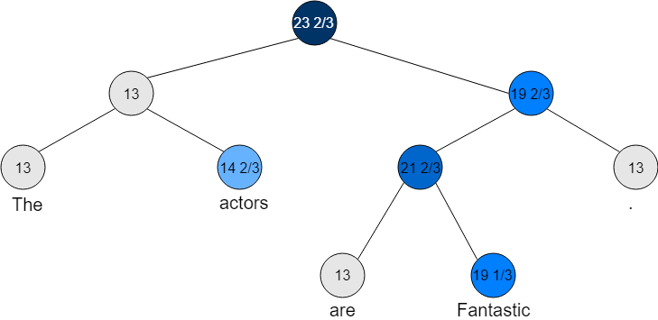
\includegraphics[width=1\textwidth]{literature_review/treebank.png}}
\caption{\label{fig:treebank} A labelled movie review in the Stanford NLP Sentiment Treebank \cite{stanfordSentiment2013}.}
\end{figure}

The Stanford NLP (Natural Language Processing) Group's Sentiment Analyser \cite{stanfordSentiment2013} introduced a Recursive Neural Tensor Network (RNTN) along with a Sentiment Treebank. The Sentiment Treebank extended the corpus of movie reviews originally collected by Pang and Lee \cite{panglee2004}. The sentences in the movie review corpus were relabelled at a phrase level, producing a sentiment labelled parse-tree for each review (Figure ~\ref{fig:treebank}). The Sentiment Treebank produced has more finely grained sentiment labels than the original corpus. It improved how the compositional effects of sentiment in language were captured. For example, a word may be positive in one context but negative in another. In this sentence, \emph{'The phone has a really long battery life'}, long is positive. However in this sentence, \emph{'The website took so long to load'}, long is negative. All classification models trained with the Sentiment Treebank saw a significant increase in accuracy. These included Naive Bayes, Support Vector Machines, and other recursive neural networks. The RNTN achieved the highest accuracy of 85.4\% in single sentence positive/negative classification.

\section{Recommender Systems}

%SL: I think you may be able to move some of the introduction section on RecSys to here. There is a section which gives an overview of collab filtering and Content-based rec which could go here, there is also detail on CORe which could probably be moved here too. 

Recommender systems provide suggestions for items that are most likely to be of interest to a particular user \cite{Ricci2015}. They recommend based on user behaviours and preferences, such as explicit user ratings and reviews of products, and implicit user clicks and view times. Some popular recommender systems include Netflix which recommends films and television programmes, Facebook which recommends new friends and content via your news feed, and TripAdvisor which recommends hotels. Recommender systems try to help consumers overcome information overload. There are two main methods that recommender systems use to generate recommendations, Collaborative Filtering methods and Content-Based recommender methods. 

Collaborative Filtering methods analyse the behaviour of a collection of users and use this information to make recommendations based upon what users similar to the current user have liked. The basic idea is that if we know two users have the same opinion on one item, then they are more likely to have the same opinion on another item. The correlation between users is used to make predictions.

Content-Based (CB) recommender methods use the descriptive features of items, and the preferences of individual users. Information about each user and the content information about each item is combined to make recommendations. CB methods recommend items similar to items the user liked or purchased in the past.

Context-aware recommender systems use contextual information to improve their recommendations. This contextual information could be time, location, company etc. The concept is that the same user could prefer different items under different conditions.

A number of recommender systems that focus on hotels have been proposed in the literature. A. Levi, O. Mokryn, C. Diot, and N. Taft proposed a recommender system that specifically focuses on hotel recommendations. This is a cold start, context-based hotel recommender system, which uses the text of online reviews from Tripadvisor and Venere as its main data \cite{levi2012}. The system asks the user to identify their trip intent (business, family, etc), nationality and preferences for certain hotel features (location, service, food, etc). Hotels are recommended based on the sentiment of reviews of users who have similar context information. The sentiment score is calculated with a lexicon based approach. Adjectives that reviewers use to express opinions are considered 'opinion words'. Opinion words are extracted for each feature from every sentence of a review. A sentiment score is calculated for each feature using the lexicon. An overall feature sentiment score is then calculated based on information about the user. The feature sentiment score is combined with the scores based on the user's trip intent and nationality to produce a hotel score. A. Levi, O. Mokryn, C. Diot, and N. Taft reported that users were 20\% more satisfied with their recommendations. This is a promising result for this research. The hope is that incorporating review-like tweets into the CoRE recommender will also increase user satisfaction. 
%SL: How is sentiment incorporated? This will be useful to reflect on or compare to for our approach

Another recommender system that targets hotels was proposed by K. Lin, C. Lai, P. Chen, and S. Hwang \cite{lin2015}. It also uses hotel reviews collected from TripAdvisor. The system tracks the user's gestures on a mobile device to identify what part of the review the user has focused on or 'seriously read'. Feature extraction is used to extract the aspects of hotels (e.g room, food, price etc) the user considers important, and build a user interest profile. Hotels are recommended based on the user profile. The score is calculated based on the sentiment of the reviews about the aspects of the hotels the user prefers.

J. Chang, C. Tsai, and J. Chiang \cite{chang2018} proposed a hotel recommendation system that uses a combination of Twitter and Yelp data. They use a collaborative filtering method. The idea is that Twitter provides limited information on its own, but when combined with Yelp, which has explicit user ratings, can achieve better performance in a recommender system. User posting behaviour vectors are generated for both Twitter and Yelp and are combined to make recommendations.

T. Takehara and S. Miki, and N. Nitta  and N. Babaguchi, propose a rule-based method of extracting context information from Twitter for use alongside a restaurant recommender system \cite{takeharaContext2012}. Relevant keywords are extracted from reviews from Tabelog \footnote{\url{https://tabelog.com}} (a Japanese review site) and are used to search Twitter for the contextual information. Nouns are extracted from Tabelog using part-of-speech tagging. Those characteristically used for assessing restaurants in each area are selected as keywords and categorised as area related keywords or restaurant related keywords. Finally, tweets containing more than two nouns from each set of keywords (area and restaurant) are selected as the contextual information and are displayed alongside the restaurant recommendations.

CoRE \cite{core2019} is a Cold Start Resistant and Extensible Recommender system. It is a hotel recommender system that makes use of collaborative filtering, content-based recommendation and contextual suggestion. The algorithm is designed to work in cold start situations and to be easily extensible. A cold start situation is when you need to make recommendations for a new user that you have no previous information on. CoRE is made up of three models, a user model, a segment model and a context model. Each model is generated as a weighted feature vector. A centroid vector is then calculated, and a weighting is applied to determine the effect of each model. The cosine similarity between the vector of each hotel and the centroid vector of the user is then calculated, and the hotels are ranked based on this score.

%ANI: Do you mean a centroid vector (i.e. centroid of a user model, a segment model and a context model) is calculated to get the final representation of a user vector/model for a specific user, which is then compared (by cosine similarity) with each hotel vector? If it is so then (user specific) personalization is already there in CoRE and you are not introducing an extra personalization by adding a fourth model to CoRE because this sentiment analysis is hotel specific and not user specific. Probably you do not want to add a fourth model to CoRE user model. You may want to update the vector representation of each hotel in Dublin by adding an extra feature (sentiment score) of that hotel. Because adding a hotel specific score to a user model will act as a constant and it won't change the performance.
%SL: Agreed, I think sentiment is likely to be used to re-rank (or influence the initial ranking of) the hotels for a user, rather than being incorporated as an extra model for the user. 

%CoRE is easily extensible by the addition of more models. This research aims to improve the performance of this recommender system by adding a fourth model, which will use a sentiment score for each hotel, generated through the analysis of review-like tweets. 

\section{Summary}

%SL: You would normally have a section at the end of this chapter which summarises the "influences from the state of the art" - that means what are the key things you took from the state of the art that influenced you research, e.g. a particular algorithm to use, a particular approach to recommendation that was demonstrated to be best, avoiding something because it has previously been shown not to work etc. 

In this chapter the background literature relating to this project has been discussed. A series of text classification techniques were researched. For classifying tweets there was no obvious winner in terms of performance. A. Bermingham and A. F. Smeaton found that the Multinomial Naive Bayes Classifier outperformed the Support Vector Machine Classifier in classifying tweets and short-form reviews \cite{Berm2010}. Ankit and N. Saleena, and M. Kanakaraj and R. M. R. Guddeti both found Ensemble Classification Methods outperformed base classifiers in classifying tweets \cite{Ankit2018,Kanakaraj2015}. The study most similar to ours, deals with airline reviews \cite{Rane2018}. A. Rane and A. Kumar found that the Random Forest Classifier followed closely by the Support Vector Machine achieved the best performance. It will be interesting to see which if any of these results will be confirmed by our research.

The majority of the tweet classification studies focus on classifying the sentiment of tweets. It was hard to find any studies about classifying tweets as reviews. That is the area that this project will focus on. 

This chapter also outlined some techniques used in hotel recommender systems. The most promising result came from A. Levi, O. Mokryn, C. Diot, and N. Taft who demonstrated that incorporating TripAdvisor reviews into their hotel recommender system increased the average user satisfaction.

% Found the Stanford NLP
% Feature Representations





